\documentclass{beamer}

\usepackage{beamerthemesplit}

\title{Zero to Root in 12 Months}
\subtitle{Training and Utilizing Junior Sysadmins in Higher Education}
\date{\today}
\author{Spencer Krum, William Van Hevelingen}

\begin{document}

\frame{\titlepage}

% Slide 
\section{Introduction}
\subsection{Presenters}
\frame 
{
    \frametitle{Presenters}
        \begin{columns}[c]
        \column{.5\textwidth}
        \begin{center}
        Spencer Krum\\
        nibz@cat.pdx.edu\\
        \end{center}
        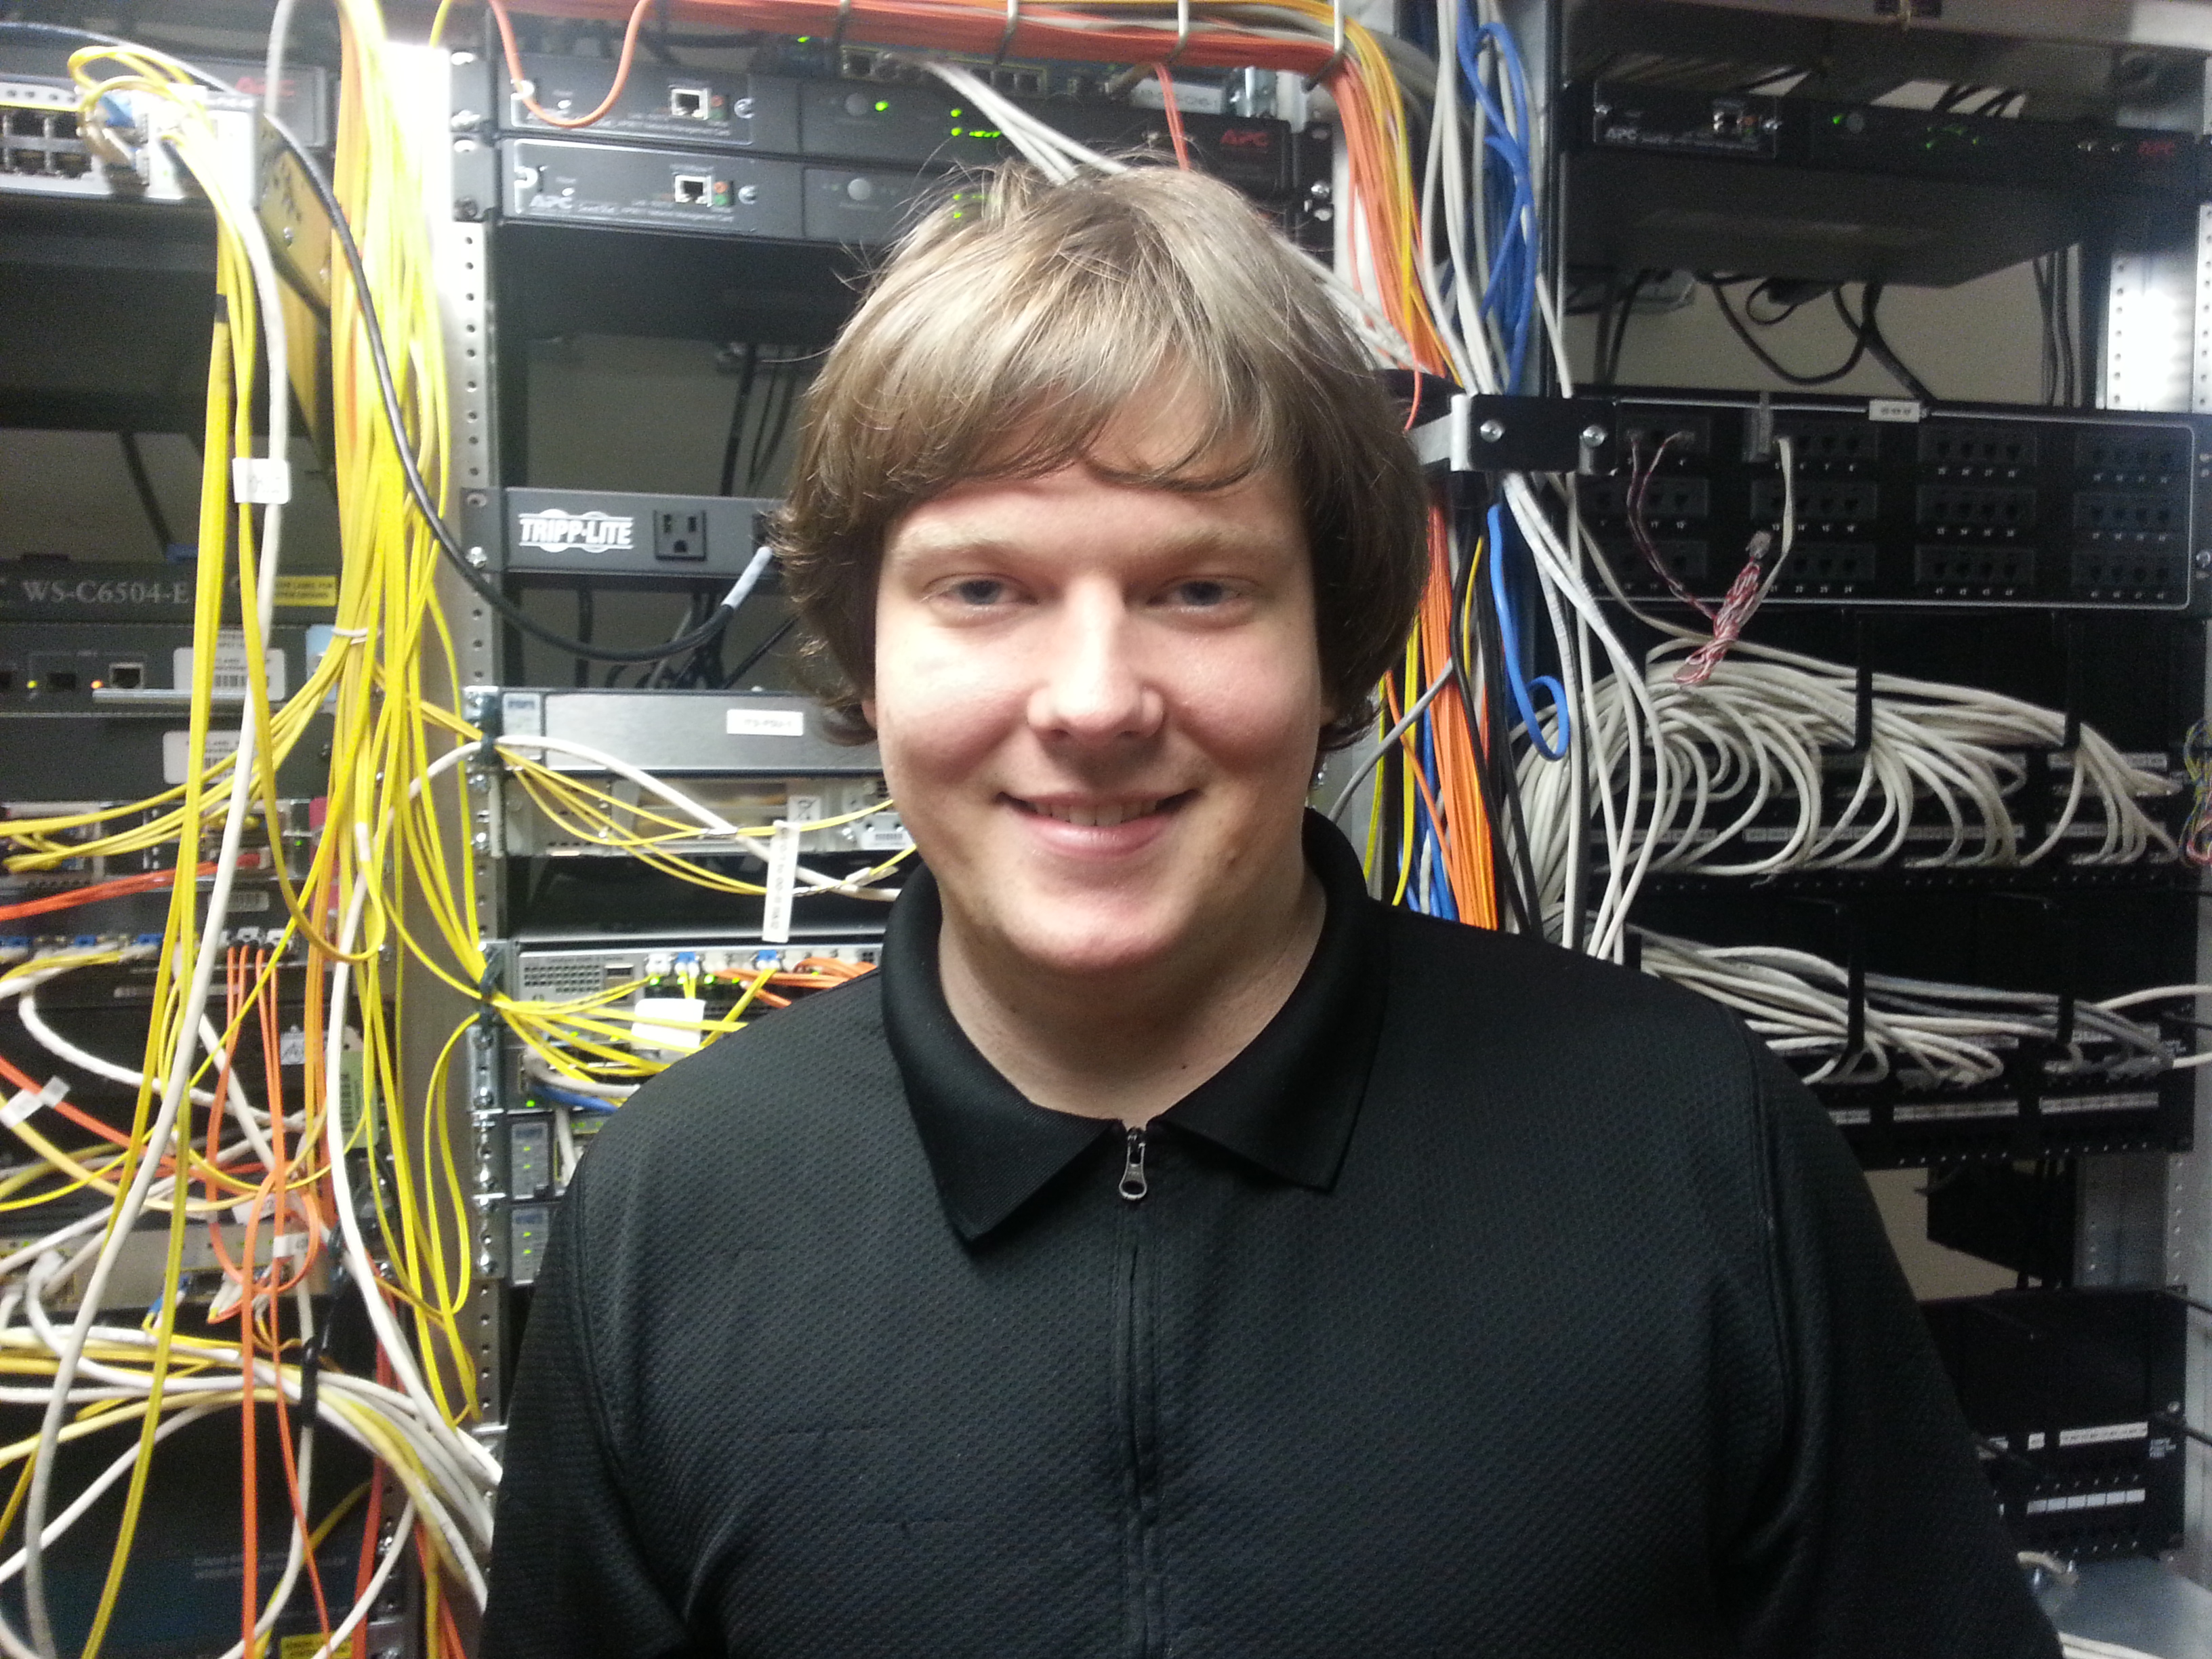
\includegraphics[width=1\textwidth]{spencer.jpg}
        
        \column{.5\textwidth}
        \begin{center}
        William Van Hevelingen\\
        blkperl@cat.pdx.edu\\
        \end{center}
        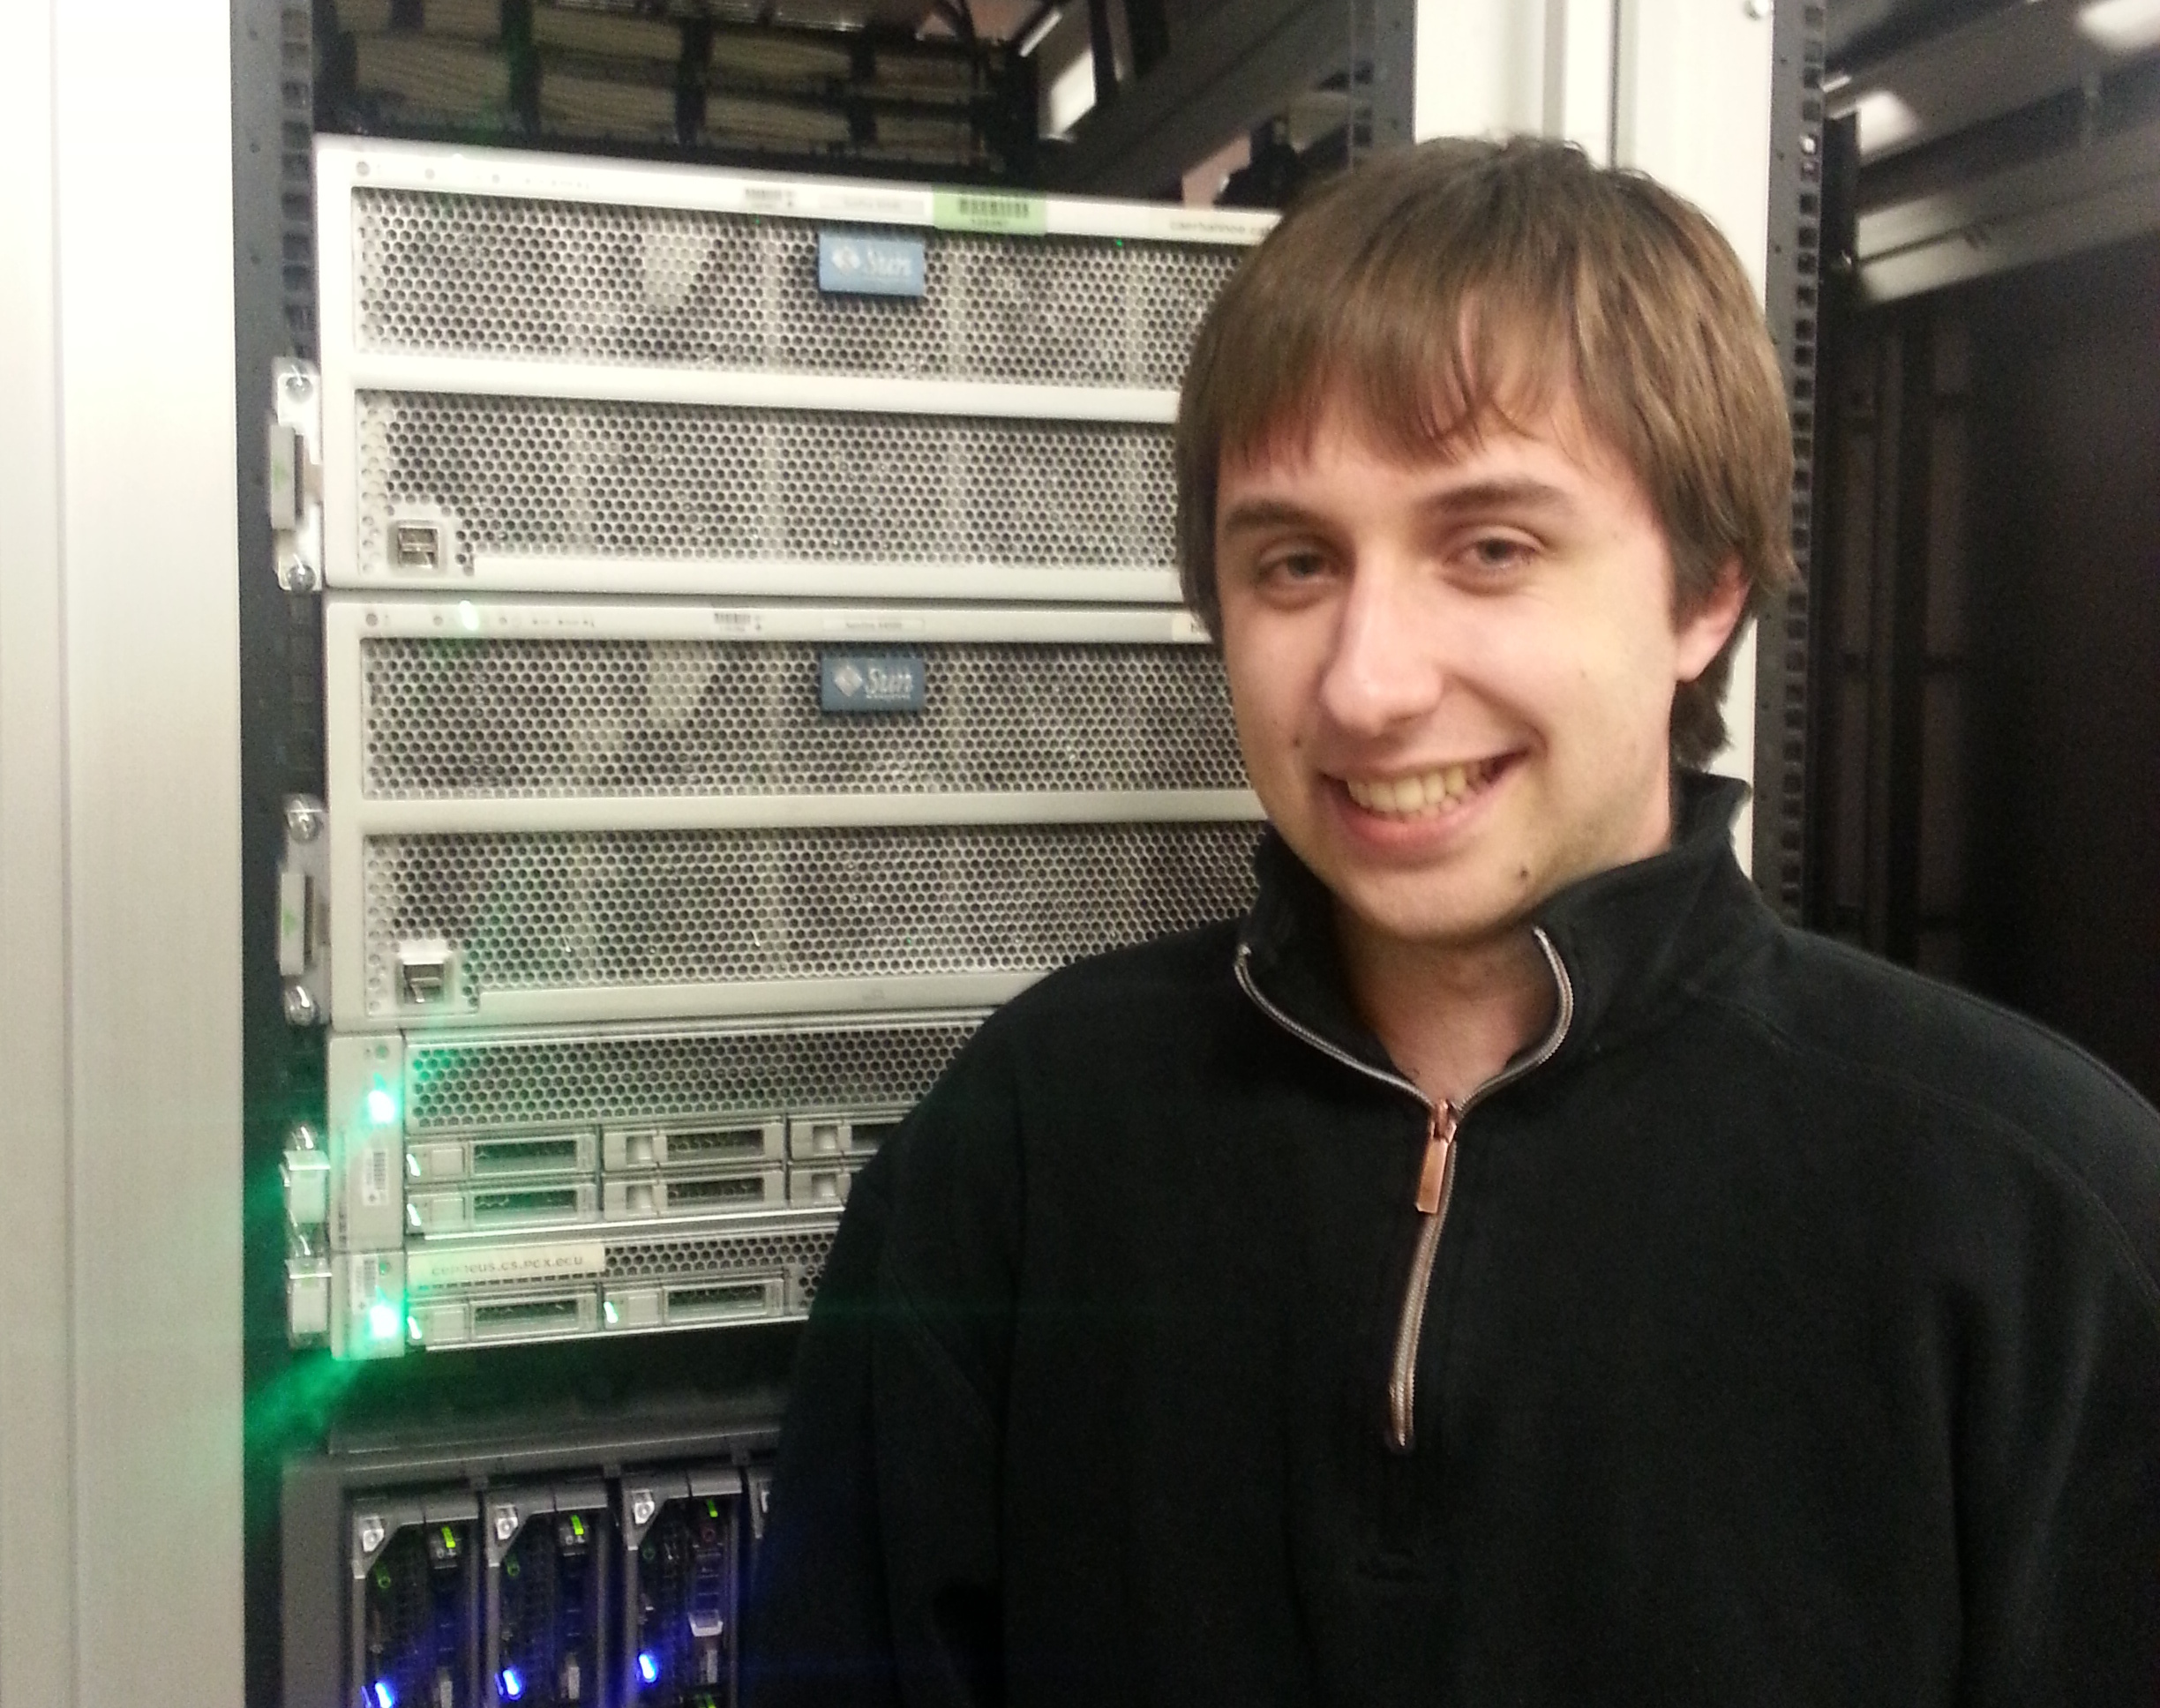
\includegraphics[width=1\textwidth]{blkperl.jpg}
        \end{columns}
}
% Slide 
\subsection{Agenda}
\frame
{
    \frametitle{Agenda}
    \begin{itemize}
        \item Computer Action Team introduction and history
        \item Braindump program
        \item Utilization
        \item Personal Stories
    \end{itemize}
}

% Slide
\section{Computer Action Team}
\subsection{Stats}
\frame
{
    \frametitle{Stats}
    \begin{itemize}
        \item 4 Buildings
        \item 5K users
        \item 600 Workstations, 100 Servers
        \item 7 general use computer labs
        \item Manage hundreds of commercial and OSS software pkgs
        \item 1854 active networking jacks
        \item Multiple 10GigE links to the internet
    \end{itemize}

}

\subsection{Operating Systems}
\frame
{
    \frametitle{Operating Systems}
    \begin{itemize}
        \item Windows
        \item Ubuntu
        \item RedHat/Centos
        \item Solaris/Derivatives
    \end{itemize}
}

% Slide
\subsection{CAT Services}
\frame
{
    \frametitle{CAT Services}
    \begin{itemize}
        \item Web
        \item License management
        \item Network homedirs
        \item Bulk storage over NFS/Samba
        \item Database (mysql/postgres)
        \item Project Management \& VCS
        \item Backups
        \item VPN
        \item Networking
        \item Mail
    \end{itemize}

}

% Slide
\section{Braindump}
\subsection{Background}
\frame
{
    \frametitle{Background}
    \begin{itemize}
        \item Founded in early 90s by Janaka Jayawardena, Director of IT for Engineering
        \item Originally a means by Janaka to grow UNIX hackers that got out of hand.
        \item In-house apprenticeship program to bring student volunteers into sysadmin and other IT roles.
        \item Hire them later (once they know what they are doing)
    \end{itemize}
}

% Slide
\subsection{Particulars}
\frame
{
    \frametitle{Particulars}
    \begin{itemize}
        \item 1+ yr program
        \item Open to any PSU student/staff
        \item Friday nights, 6pm-10pm
        \item 4 hours helpdesk volunteering a week
        \item Time, as needed, spent working on learning and projects.
    \end{itemize}
}

% Slide
\subsection{Typical Braindump}
\frame
{
    \frametitle{Typical Braindump}
    \begin{itemize}
        \item Senior CAT speaks
        \item 3-4 hour presentation on a technical subject, usually part of a "track"
        \item Informal, questions and tangents throughout
        \item A Braindump cohort begins with about 60 people but attrition soon sets in.
    \end{itemize}
}

% Slide
\frame
{
        \includegraphics[width=1\textwidth]{ataris_full.jpg}
}

% Slide
\frame
{
        \includegraphics[width=1\textwidth]{braindump_anakha.jpg}
}

% Slide
\subsection{Catacombs}
\frame
{
    \frametitle{Catacombs}
    \begin{itemize}
        \item Sandbox environment
        \item Physical equipment
        \item Braindump group has total control of hardware and network
        \item Goal is to replicate production
        \item Install operating systems and set up services
    \end{itemize}
}

% Slide
\frame
{
        \includegraphics[width=1\textwidth]{combs1.jpg}
}

% Slide
\frame
{
        \includegraphics[width=1\textwidth]{combs2.jpg}
}


% Slide
\subsection{Scratching Post}
\frame
{
    \frametitle{Scratching Post}
    \begin{itemize}
        \item Office hours
        \item Student driven
        \item Senior CAT sits down with students for 2 or more hours per week
        \item Place to drill down into internals
        \item Different teaching format for different types of learning
    \end{itemize}
}

% Slide
\frame
{
        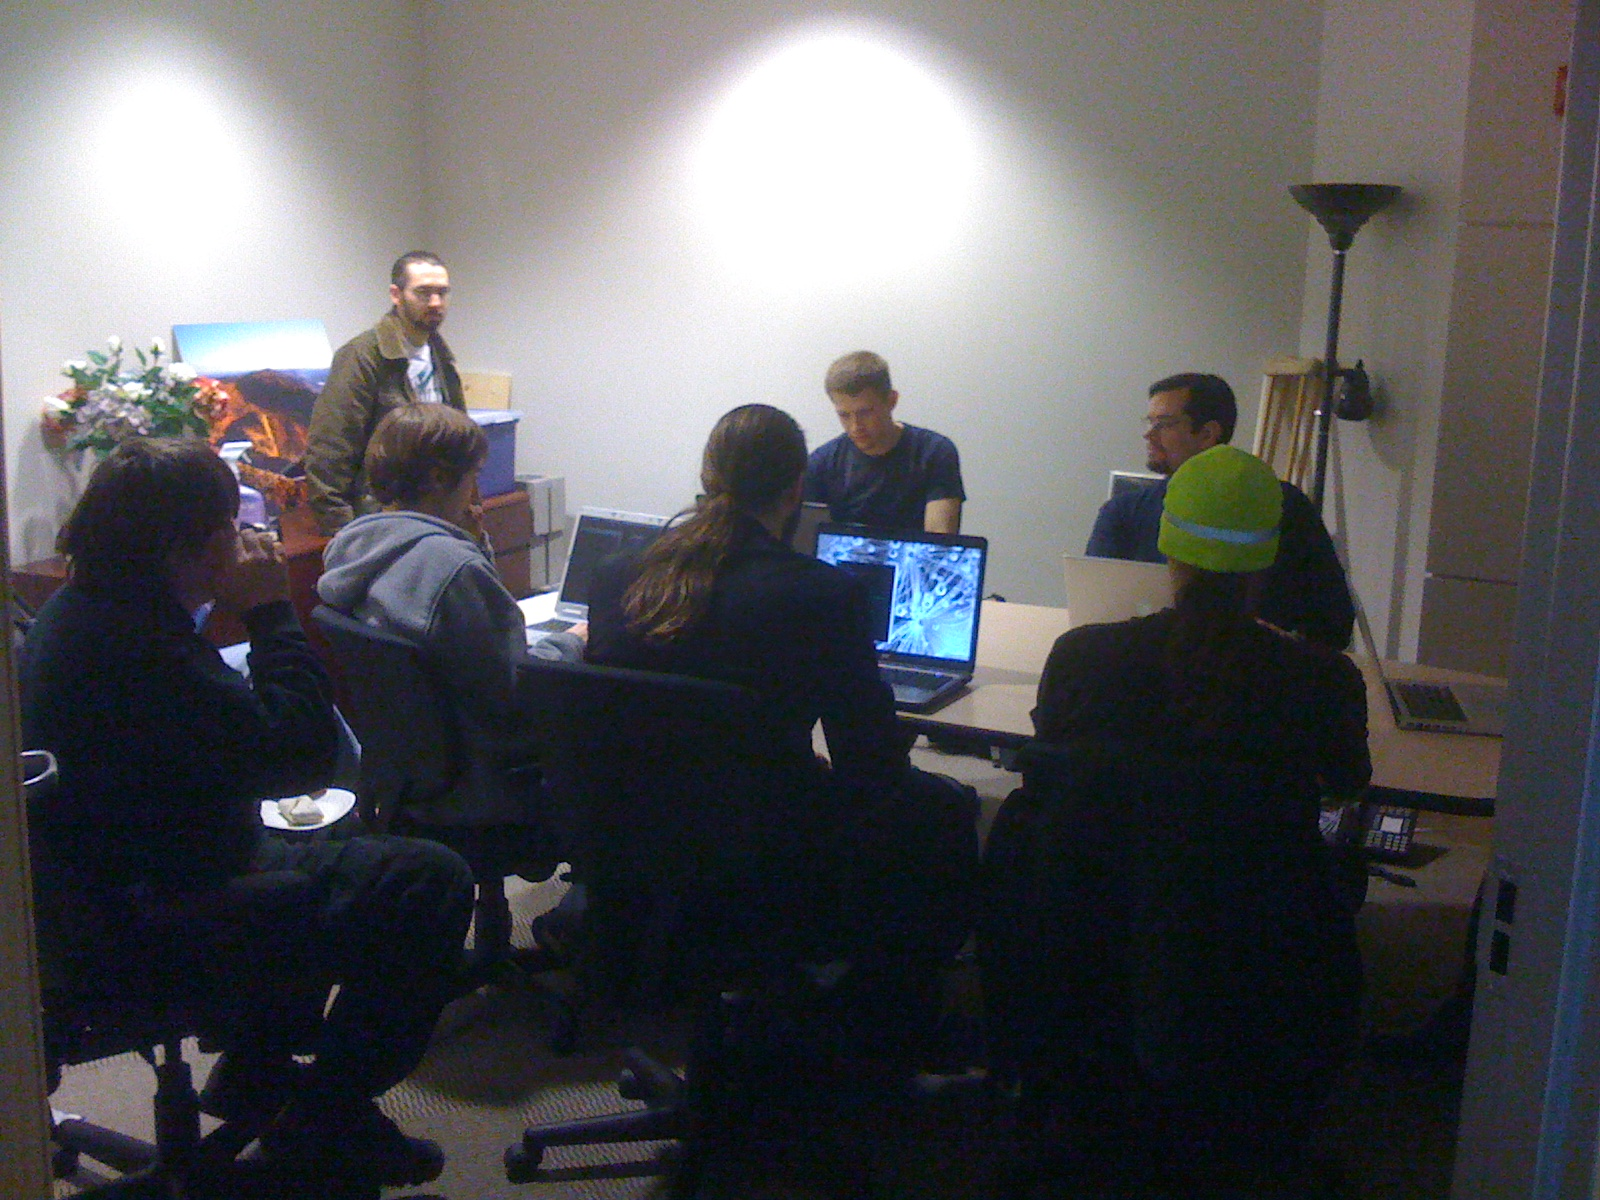
\includegraphics[width=1\textwidth]{scratching.jpg}
}


% Slide
\subsection{Mentor Session}
\frame
{
    \frametitle{Mentor Session}
    \begin{itemize}
        \item Small groups of about 10 students
        \item Two mentors
        \item Takes place in a lab environment
        \item Tutorial on the basics
      \begin{itemize}
          \item CAT Environment
          \item Shell
          \item SSH
          \item Basic Scripting
          \item IRC
      \end{itemize}
    \end{itemize}
}

% Slide
\section{Utilization}
\subsection{Root}
\frame
{
    \frametitle{Root}
    \begin{itemize}
      \item "You let students have root?!" \\
    \end{itemize}
}

% Slide
\subsection{Root}
\frame
{
    \frametitle{Root}
    \begin{itemize}
      \item "Yes" 
      \item "But not at first" 
    \end{itemize}
}

% Slide
\subsection{What do they provide for us}
\frame
{
    \frametitle{What do they provide for us}
    \begin{itemize}
      \item First tier support in person and via phone and email
      \item Password resets
      \item Lab monitoring
    \end{itemize}
}

% Slide
\frame
{
        \includegraphics[width=1\textwidth]{desk.jpg}
}

% Slide
\subsection{Self selection}
\frame
{
    \frametitle{Self selection}
    \begin{itemize}
      \item Students who want to give back to production will self select
      \item Usually about 20\% of the braindump will do this
    \end{itemize}
}

% Slide
\frame
{
        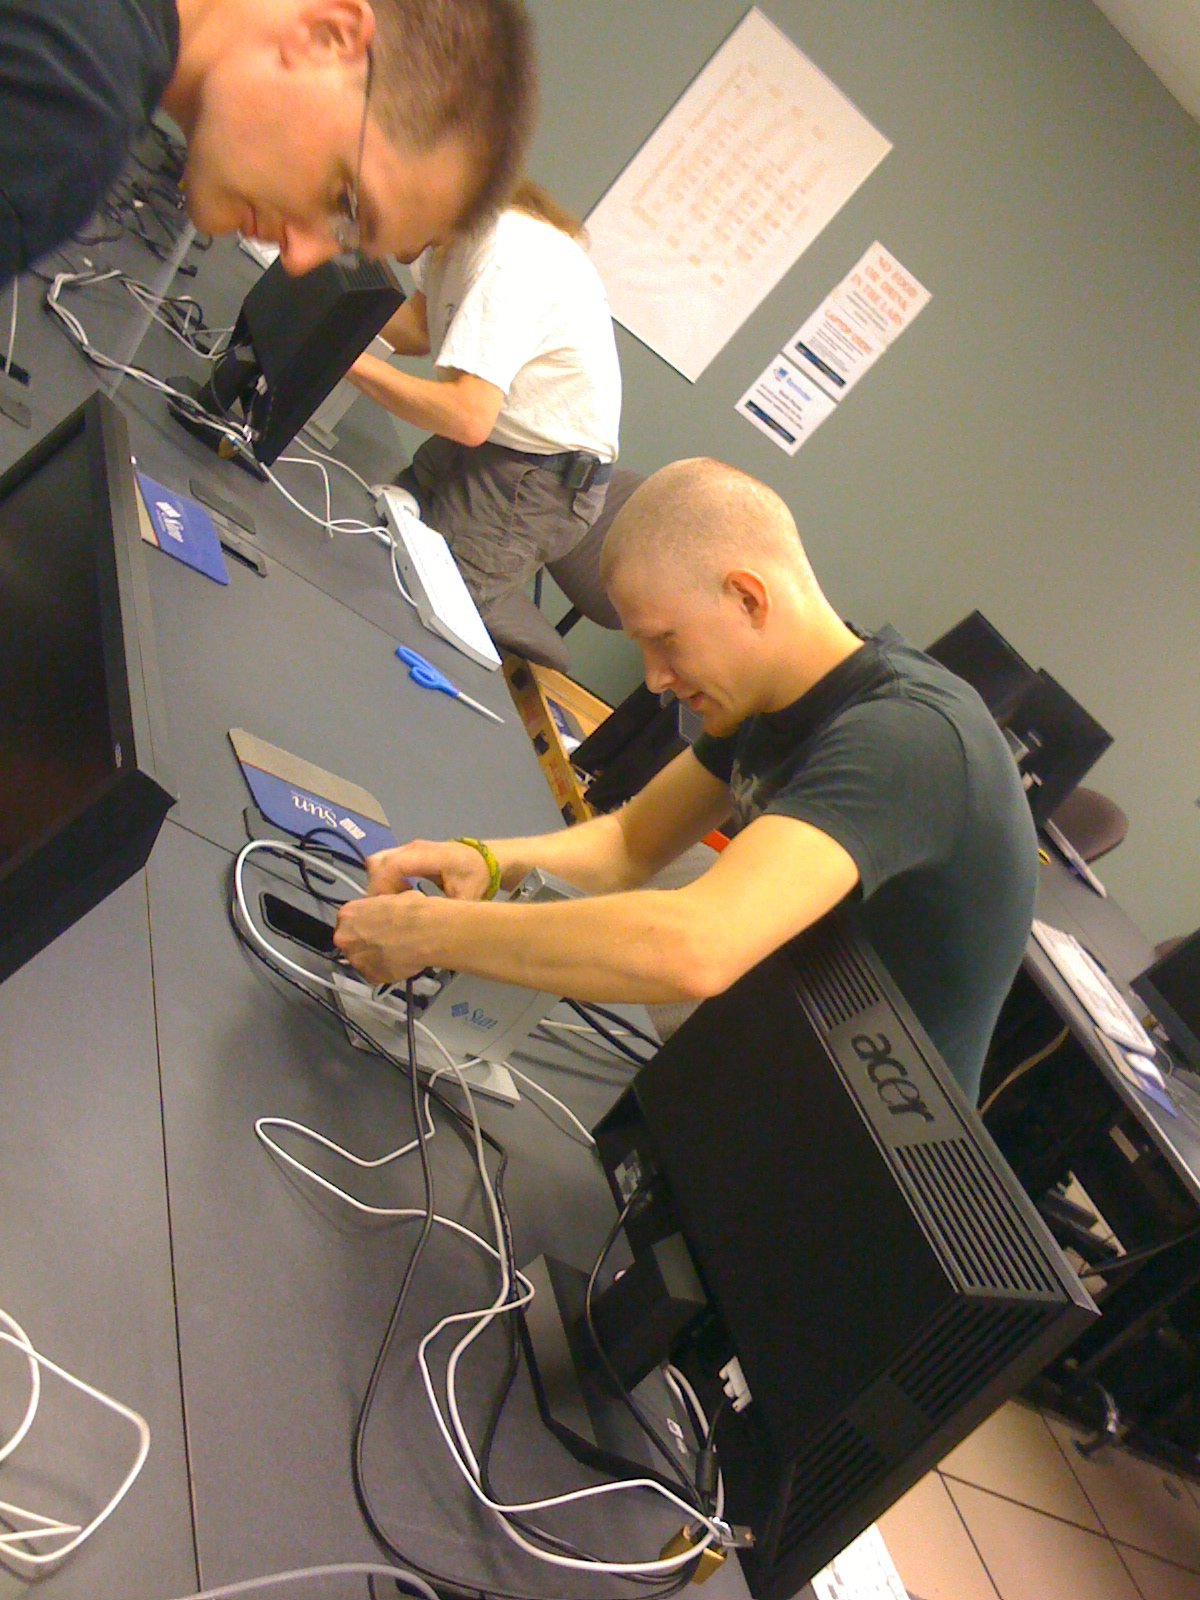
\includegraphics[width=1\textwidth]{deskcats.jpg}
}

% Slide
\frame
{
    \frametitle{What does that looks like}
    \begin{itemize}
      \item Self selecting students will come to scratching post and team meetings
      \item Small tasks will be assigned that can be performed as a user
    \end{itemize}
}

% Slide
\frame
{
    \frametitle{What do they provide for us}
    \begin{itemize}
      \item Read/grep logs for general issues
      \item Analyze logs in debugging of a specific issue
      \item Write utility and status scripts
      \item Second tier support via email and house calls
      \item Build, package, install software
      \item Monitor systems for runaway processes
      \item Basic commits to puppet, nagios, and graphite
      \item Commits to internal web applications
    \end{itemize}
}


% Slide
\frame
{
    \frametitle{More self selection}
    \begin{itemize}
      \item 3 months in, students are let into the combs
      \item More attrition
      \item Motivated students will learn and/or demonstrate ability to install operating systems and setup services
    \end{itemize}
}

% Slide
\frame
{
    \frametitle{What do they do for us}
    \begin{itemize}
      \item Test upgrades to services
      \item Database
      \item Web applications
    \end{itemize}
    \begin{itemize}
      \item Test and evaluate new services to deploy
    \begin{itemize}
      \item LDAP/Kerberos
      \item Hadoop
    \end{itemize}
      \item Significant changes to puppet, nagios, graphite
      \item Extend infrastructure
    \end{itemize}
}

% Slide
\subsection{Rooting}
\frame
{
    \frametitle{Rooting}
    \begin{itemize}
      \item At 6 months in, some students will have demonstrated:
      \begin{itemize}
        \item Personal integrity
        \item Participation at team meetings
        \item Basic competence with the technologies we use
      \end{itemize}
      \item If these criteria are met we usually give them root access to the 'client' systems.
    \end{itemize}
}

% Slide
\frame
{
    \frametitle{Rooting}
    \begin{itemize}
      \item Student rooters get:
      \begin{itemize}
        \item workstations and services 
        \item not fileservers
        \item not ldap or dns
        \item some, less critical, database servers
        \item This is to minimize 'blast zone' in case of a screwup
      \end{itemize}
      \item Windows is a bit different because they have fewer services and kerberos
    \end{itemize}
}

% Slide
\frame
{
    \frametitle{What do they do for us}
    \begin{itemize}
      \item OS installs/reinstalls
      \item OS Upgrades/Patches
      \item Networking
      \item VM management
      \item Puppet development, testing environments
      \item Restores from backup
      \item Mail debugging
      \item General Debugging
    \end{itemize}
}

% Slide
\frame
{
        \includegraphics[width=1\textwidth]{droog.jpg}
}

% Slide
\frame
{
        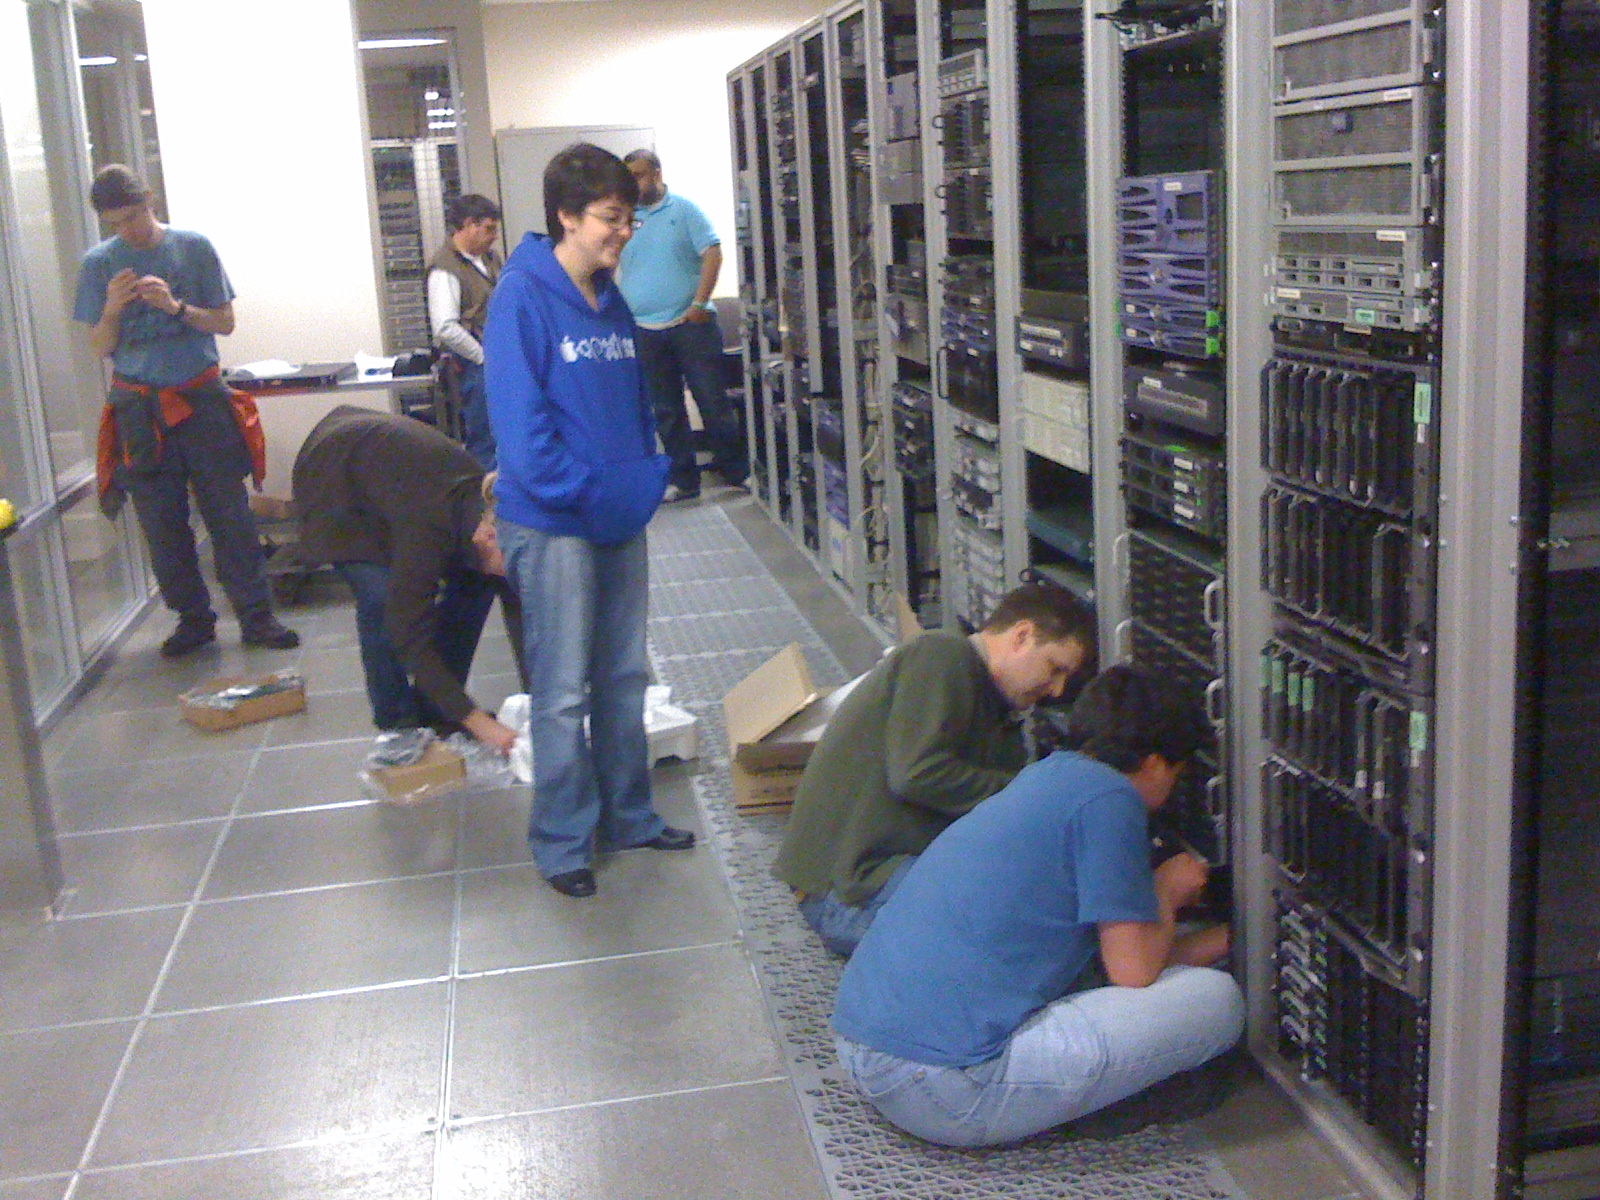
\includegraphics[width=1\textwidth]{dcops.jpg}
}

% Slide
\frame
{
    \frametitle{Further Promotion}
After another six months or so, we sometimes promote them again to full root.\\

This means fileservers, puppet masters, authoritative dns servers, ldap servers, and database servers.\\
}

% Slide
\frame
{
    \frametitle{What do they do for us}
    \begin{itemize}
      \item At this level they are on-par with FTEs
      \item Exports list
      \item Filesystem create/destroy
      \item Group membership
      \item Full puppet production commit access
      \item DNS zones
    \end{itemize}
}

% Slide
\frame
{
        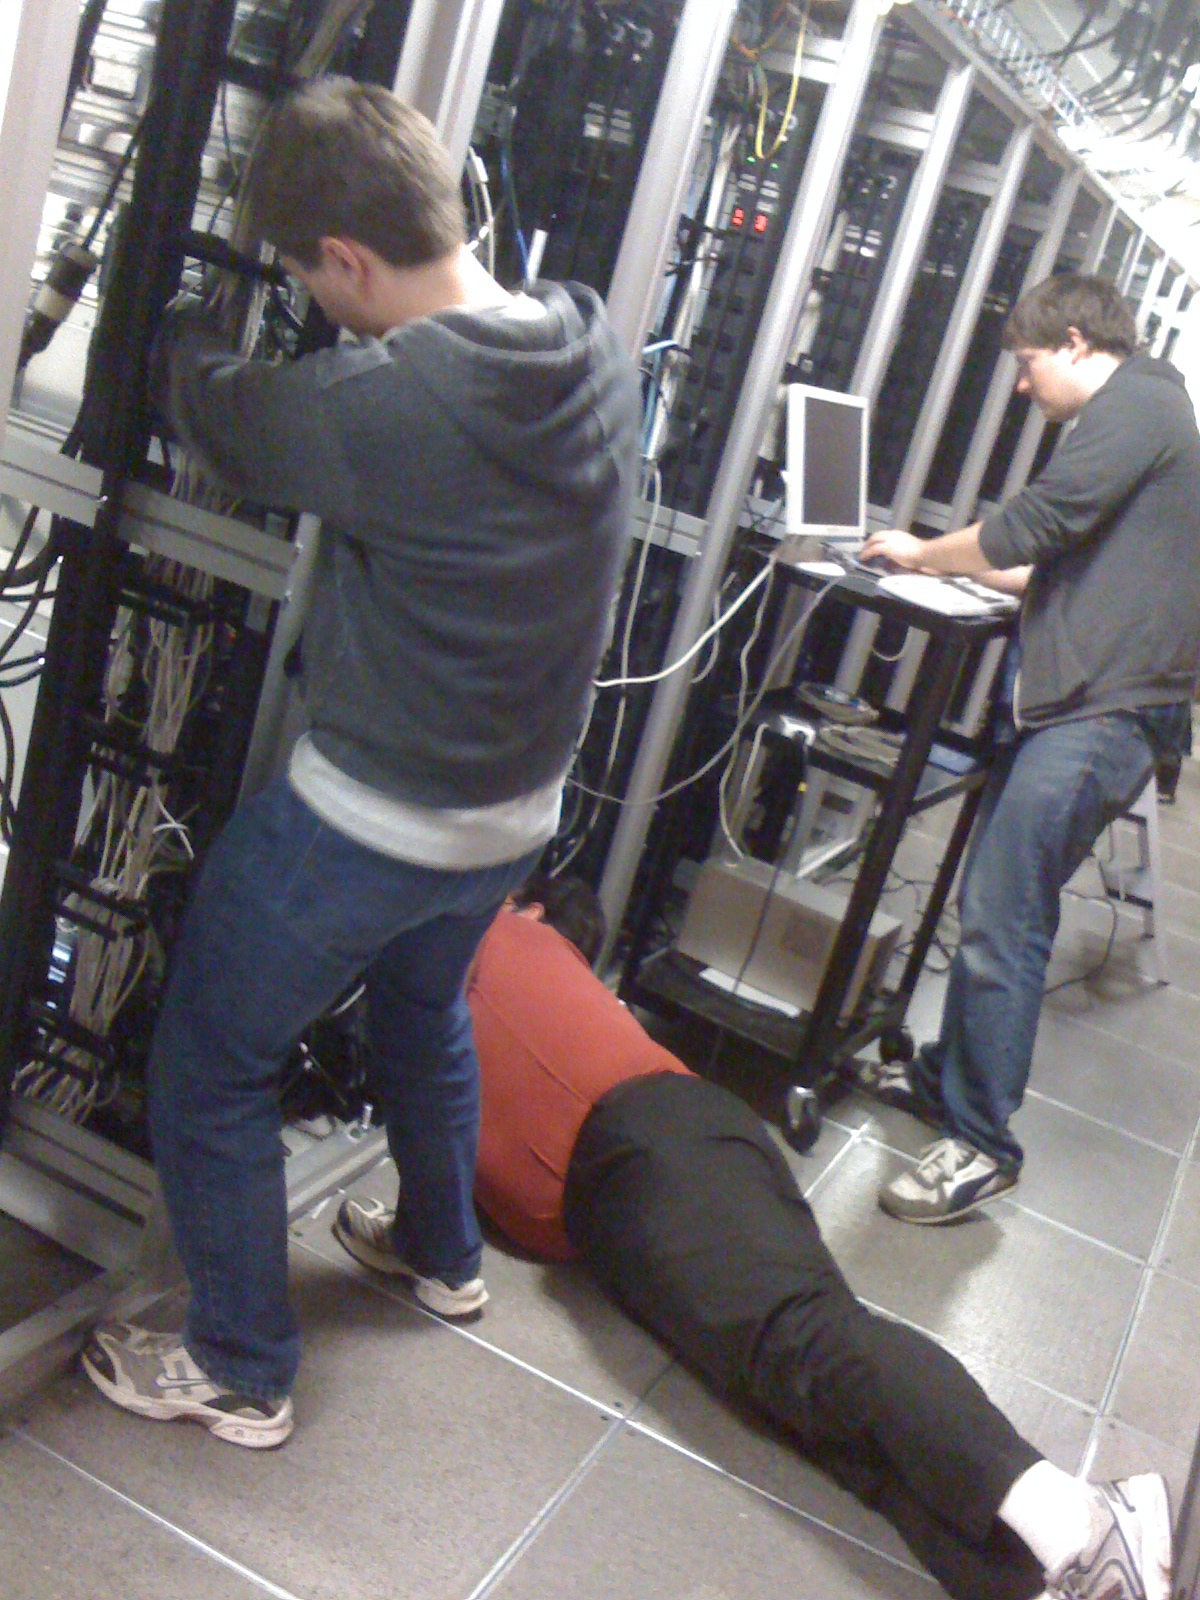
\includegraphics[width=1\textwidth]{claws.jpg}
}

% Slide
\subsection{Other Tracks}
\frame
{
    \frametitle{Other tracks}
    \begin{itemize}
      \item Networking team
    \begin{itemize}
      \item IOS ninja and debug networking for users
    \end{itemize}
      \item Syndicat
    \begin{itemize}
      \item Web development, mostly PHP
    \end{itemize}
      \item User Support
    \begin{itemize}
      \item Advanced user support
    \end{itemize}
    \end{itemize}
}

% Slide
\subsection{Stories}
\frame
{
    \frametitle{Stories}
    Stories and Thank You
}

\end{document}

